
%(BEGIN_QUESTION)
% Copyright 2012, Tony R. Kuphaldt, released under the Creative Commons Attribution License (v 1.0)
% This means you may do almost anything with this work of mine, so long as you give me proper credit

Some precision manometers are equipped with a {\it vernier} scale in order to make very precise measurements of liquid column height.

\vskip 10pt

Interpret the reading shown on this mercury manometer.  Note: the ``hairline'' on the moving vernier scale is adjusted to the meniscus height by a screw prior to taking the reading:

$$\includegraphics[width=15.5cm]{i01129x01.eps}$$

\underbar{file i01129}
%(END_QUESTION)





%(BEGIN_ANSWER)

A pressure of {\bf 45.19 cm} of mercury is shown on this manometer.
 
%(END_ANSWER)





%(BEGIN_NOTES)


%INDEX% Measurement, pressure: manometer
%INDEX% Mechanics, reading an analog scale (vernier manometer)

%(END_NOTES)


